\documentclass[xcolor=dvipsnames]{beamer}
\usepackage{amsfonts, epsfig, xspace, relsize}
\usepackage{algorithm,algorithmic, graphicx}
\usepackage{pstricks,pst-node}
\usepackage{multimedia}
\usepackage{enumerate}
\usepackage[normal,tight,center]{subfigure}
\setlength{\subfigcapskip}{-.5em}
\usepackage{beamerthemesplit}
\usepackage{mathtools}
\DeclareMathOperator*{\plim}{plim}
\DeclareMathOperator*{\argmin}{argmin}
\usepackage{xcolor}
\usepackage{fancyvrb}
\usepackage{framed,color}
\definecolor{shadecolor}{rgb}{0.8,1,0.5}
\usepackage{amsmath}% http://ctan.org/pkg/amsmath
\usepackage[retainorgcmds]{IEEEtrantools}% http://ctan.org/pkg/ieeetran
\newcommand{\non}{\IEEEnonumber*}
\setbeamertemplate{caption}[numbered]
\usepackage{fontspec}  %加這個就可以設定字體
\usepackage{xeCJK}       %讓中英文字體分開設置
%\setromanfont{LiHei Pro} % 儷黑Pro
\newCJKfontfamily{\K}{標楷體}
\newCJKfontfamily{\H}{微軟正黑體}
\setmonofont[Scale=0.8]{Courier New} % 等寬字型
\setCJKmainfont{細明體} %設定中文為系統上的字型,而英文不去更動,使用原TeX字型
\XeTeXlinebreaklocale "zh"             %這兩行一定要加,中文才能自動換行
\XeTeXlinebreakskip = 0pt plus 1pt     %這兩行一定要加,中文才能自動換行
%\usetheme{lankton-keynote}
\usetheme{Madrid}
\usecolortheme[named=BrickRed]{structure}
\author[蔡佳泓]{\K 蔡佳泓}

\title[Statistical Methods for Social Sciences]{Regression Analysis\\
\smallskip
{\small {Simple Linear Regression}}}
\date{June 3, 2015} %leave out for today's date to be insterted
\institute[ESC \& GIEAS]{\H 國立政治大學東亞所}
\begin{document}
\maketitle
\tableofcontents
\section{OLS}
\subsection{OLS的原理}
\begin{frame} \frametitle{\H 為何使用OLS}
\begin{itemize}
\item OLS代表Ordinary Least Squares,也就是最小平方法。
\item 假設$ \{\tilde{\beta}_{0},\tilde{\beta}_{1}\} $是$ \{\beta_{0},\beta_{1}\} $的可能值之一,OLS迴歸的目的是找到最小化以下模型的$ \{\hat{\beta}_{0},\hat{\beta}_{1}\} $:
\medskip
\begin{align*}
 \{\tilde{\beta}_{0},\tilde{\beta}_{1}\}&=\argmin_{\tilde{\beta}_{0},\tilde{\beta}_{1}}\sum _{i=1}^n(y_{i}-\tilde{\beta}_{0}-x_{i}\tilde{\beta}_{0})^2 
 \end{align*}
% = \arg\min\limits_{{\tilde{\beta}_{0},\tilde{\beta}_{1}}}\sum _{i=1}^n\hat{u_{i}}^2

\medskip
\item OLS迴歸的目標就是最小化平方差和。
\item 因為平方差和容易分析而且計算,並且在某些前提成立時可達到最佳化,因此我們分析最小化平方差和。
\end{itemize}
\end{frame}
\begin{frame}\frametitle{\H 迴歸模型圖1}
\begin{figure}
\begin{center}
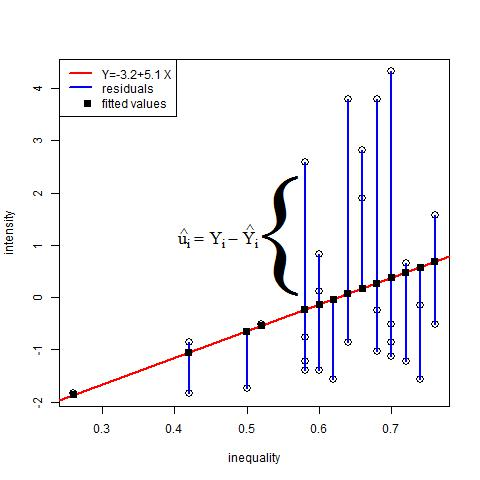
\includegraphics[scale=.45]{reg1.jpg}
\end{center}
\end{figure}
\end{frame}

\subsection{最小平方法之估計}
\begin{frame}\frametitle{\H 估計之求法}
\begin{itemize}
\item 假設隨機變數$Y$有$n$個樣本,表示為$y_{1},y_{2},\dots,y_{n}$。
\item 有一個可以摘要說明$y_{1},y_{2},\dots,y_{n}$的統計稱為$\tilde{u} $。
\item $\tilde{u} $與$y_{1},y_{2},\dots,y_{n}$之間的平方殘差和 (sum of squared residuals, SSR)之中如果找到最小化
的$\tilde{u} $,得到的係數估計有最小的變異數。
\item $\tilde{u}$可以被定義成
\begin{IEEEeqnarray*}{rCl}
\tilde{u} & = & y_{i}- \hat{y}_{i}\non \\
& = & y_{i}- \tilde{\beta}_{0}-\tilde{\beta}_{1}x_{i}\non
\end{IEEEeqnarray*}
\item OLS迴歸的目標是最小化殘差,殘差可以計算為$y_{i}- \hat{y}_{i}$,但是這會給所有的${y}_{i}  $一樣的權重。改用殘差的平方和(sum of squared residuals), 才會給離迴歸線越遠的${y}_{i}$比較大的權重,這樣才能反映離差的大小。
%\item SSR=$\sum \tilde{u}^2$,SSR越小越好。
\item 命SSR為函數$S(\tilde{u})$。要找出最小化SSR的$\tilde{u}  $
\begin{center}
$ S(\tilde{u})=\mathlarger {\sum\limits_{i=1}^n(y_{i}-\tilde{u})^2} $
\end{center}
\end{itemize}
\end{frame}
\begin{frame}\frametitle{\H 殘差函數圖}
\begin{figure}
\begin{center}
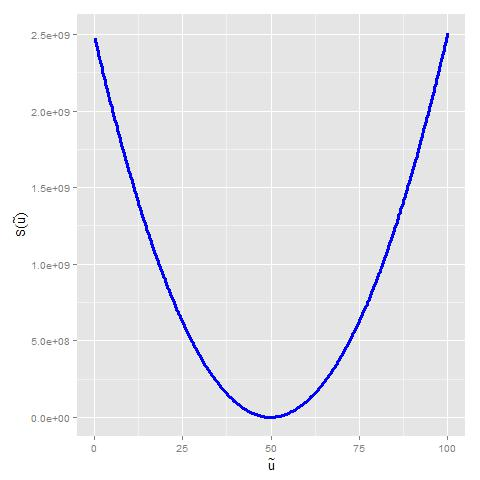
\includegraphics[scale=.45]{uplot1.jpg}
\end{center}
\end{figure}
\end{frame}
\begin{frame}\frametitle{\H 估計之求法}
\begin{itemize}
\item 進行微分:
\begin{IEEEeqnarray*}{rcl}
S(\tilde{u})& = & \mathlarger {\sum\limits_{i=1}^n(y_{i}-\tilde{u})^2} \non \\
& = & \mathlarger {\sum\limits_{i=1}^n(y_{i}^2-2y_{i}\tilde{u}+\tilde{u}^2)} \non \\
\mathlarger{\frac{\partial S(\tilde{u})}{\partial\tilde{u}}=\sum\limits_{i=1}^n(-2y_{i}+2\tilde{u})}\non
\end{IEEEeqnarray*}
\end{itemize}
\end{frame}
\begin{frame}\frametitle{\H 估計之求法}
\begin{itemize}
\item 進行微分之後,因為要求出最小化的線性函數,\\所以設定$\frac{\partial S(\tilde{u})}{\partial\tilde{u}}=0$:
\begin{IEEEeqnarray*}{rCl}
0& = & \mathlarger {\sum\limits_{i=1}^n(-2y_{i}+2\tilde{u})} \non \\
\hat{u}& \equiv & \tilde{u} = \frac{1}{n}\mathlarger {\sum\limits_{i=1}^n y_{i}} \non \\
\end{IEEEeqnarray*}
\item 樣本平均數就是最佳的殘差,也就是最小平方法的樣本統計(estimator)。
\end{itemize}
\end{frame}
\begin{frame}[fragile=singleslide]{R code}
\begin{Verbatim}[frame=single,label=R code,
formatcom=\color{blue},fontseries=b,xleftmargin=2mm]
set.seed(1000)
y1<-rnorm(1001,50,1)
u<-runif(1001,0,100)
for (i in 1:1001)
su[i]<-sum(y1-u[i])^2
up<-ggplot(dm,aes(x=residuals,y=sumofsquares))+
  geom_line(size=2,col="blue")+
  ylab(expression(paste(S(tilde(u)))))+
  xlab(expression(paste(tilde(u)))) +
  geom_hline(xintercept=0,col="red",size=1.5)
\end{Verbatim}
\end{frame}

\begin{frame}\frametitle{\H 殘差函數圖}
\begin{figure}
\begin{center}
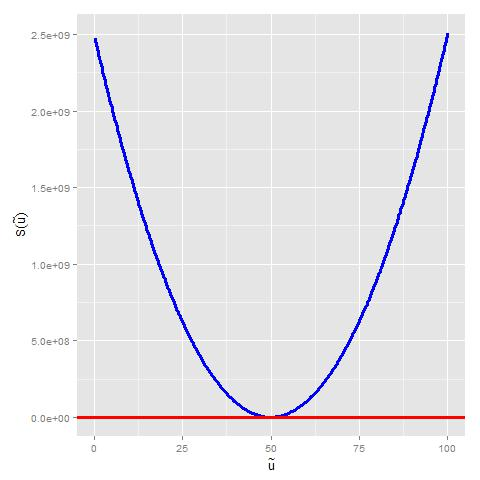
\includegraphics[scale=.45]{uplot2.jpg}
\end{center}
\end{figure}
\end{frame}
\subsection{線性的最小平方法}
\begin{frame}{\H 最小平方法的係數}
\begin{itemize}
\item 我們要找出可以最小化殘差的$\{\tilde{\beta}_{0},\tilde{\beta}_{1}\}$,做為$\{\beta_{0},\beta_{1}\}$的估計。也就是Linear Least Squares Estimator.
\begin{center}
$S(\tilde{\beta}_{0},\tilde{\beta}_{1})=\mathlarger {\sum\limits_{i=1}^n(y_{i}-\tilde{\beta}_{0}-x_{i}\tilde{\beta}_{1})^2}$
\end{center}
\item 步驟:
\begin{enumerate}
\item 首先對$\{\tilde{\beta}_{0},\tilde{\beta}_{1}\}$取微分
\item 命兩者的微分等於0
\item 求出$\{\tilde{\beta}_{0},\tilde{\beta}_{1}\}$的解。
\end{enumerate}
\end{itemize}
\end{frame}
\subsection{迴歸係數}
\begin{frame}\frametitle{\H 迴歸係數}
\begin{itemize}
\item 因為要求出最小化殘差的線性函數,而殘差可轉換成\\
$y_{i}-\tilde{\beta}_{0}-x_{i}\tilde{\beta}_{1}$,所以:
\begin{IEEEeqnarray*}{rCl}
S(\tilde{\beta}_{0},\tilde{\beta}_{1}) & = & \mathlarger {\sum\limits_{i=1}^n(y_{i}-\tilde{\beta}_{0}-x_{i}\tilde{\beta}_{1})^2} \IEEEnonumber \\
& = & \mathlarger 
{\sum\limits_{i=1}^n(y_{i}^2-2y_{i}\tilde{\beta}_{0}-2y_{i}\tilde{\beta}_{1}x_{i}+
 \tilde{\beta}_{0}^2+2\tilde{\beta}_{0}\tilde{\beta}_{1}x_{i}+
 \tilde{\beta}_{1}^2x_{i}^2)} \non \\
\end{IEEEeqnarray*}

\begin{center}
$\frac{\partial S(\tilde{\beta}_{0},\tilde{\beta}_{1})}{\partial
\tilde{\beta}_{0}}=
\mathlarger {\sum\limits_{i=1}^n(-2y_{i}+2\tilde{\beta}_{0}+2\tilde{\beta}_{1}x_{i})}$

\medskip
$\frac{\partial S(\tilde{\beta}_{0},\tilde{\beta}_{1})}{\partial
S(\tilde{\beta}_{1}})=\mathlarger {\sum\limits_{i=1}^n(-2y_{i}x_{i}+2\tilde{\beta}_{0}x_{i}+2\tilde{\beta}_{1}x_{i}^2)}$
\end{center}
\end{itemize}
\end{frame}
\subsection{first order condition}
\begin{frame}\frametitle{\H 估計之求法}
\begin{itemize}
\item 進行微分之後,因為要求出最小化的線性函數,\\所以分別設定
\begin{IEEEeqnarray*}{rCl}
0 & = & \mathlarger {\sum\limits_{i=1}^n(-2y_{i}+2\tilde{\beta}_{0}+2\tilde{\beta}_{1}x_{i})}\IEEEyesnumber*\label{eqn:first1}\\
0 & = & \mathlarger {\sum\limits_{i=1}^n(-2y_{i}x_{i}+2\tilde{\beta}_{0}x_{i}+2\tilde{\beta}_{1}x_{i}^2)}\IEEEyesnumber*\label{eqn:first2}
\end{IEEEeqnarray*}
這兩個方程式被稱為 first order condition
\end{itemize}
\end{frame}
\subsection{normal equations}
\begin{frame}\frametitle{normal equations}
根據(\ref{eqn:first1}),
\begin{IEEEeqnarray*}{c}
\hat{\beta}_{0}n= \mathlarger{(\sum\limits_{i=1}^ny_{i})-
 \hat{\beta}_{1}{(\sum\limits_{i=1}^nx_{i})}}\IEEEyesnumber*\label{eqn:normal1}\\
\tilde{\beta}_{0}=\bar{Y}-\tilde{\beta}_{1} \bar{x}\non
\end{IEEEeqnarray*}
根據(\ref{eqn:first2}),
\begin{IEEEeqnarray*}{c}
\hat{\beta}_{1}\sum\limits_{i=1}^nx_{i}^2= \mathlarger{(\sum\limits_{i=1}^nx_{i}y_{i})-
 \tilde{\beta}_{0}{(\sum\limits_{i=1}x_{i}}) }\IEEEyesnumber*\label{eqn:normal2}
\end{IEEEeqnarray*}
這兩個等式稱為normal equations

\end{frame}
\begin{frame}{OLS樣本統計}
從normal equations的第1式(\ref{eqn:normal1})可以得到:
\begin{IEEEeqnarray*}{c}
\mathlarger{\hat{\beta}_{1}=\frac{\sum y_{i}-\hat{\beta}_{0}n}{\sum x_{i}}}\IEEEyesnumber*\label{eqn:normal1.1}
\end{IEEEeqnarray*}

根據式(\ref{eqn:normal2})則可解$\hat{\beta}_{0}$為:
\begin{IEEEeqnarray*}{c}
\mathlarger{\hat{\beta}_{0}=\frac{\sum x_{i}y_{i}-\hat{\beta}_{1}\sum x_{i}^2}{\sum x_{i}}}
\IEEEyesnumber*\label{eqn:normal2.1}
\end{IEEEeqnarray*}
把(\ref{eqn:normal2.1})代入(\ref{eqn:normal1.1}):
\begin{IEEEeqnarray*}{c}
\mathlarger{\hat{\beta}_{1}=\frac{\sum y_{i}-n\frac{\sum x_{i}y_{i}-\hat{\beta}_{1}\sum x_{i}^2}{\sum x_{i}}}{\sum x_{i}}}= 
\mathlarger{\frac{n\sum x_{i}y_{i}-\sum x_{i}\sum y_{i}}{n\sum x_{i}^2-(\sum x_{i})^2}}
\IEEEyesnumber*\label{eqn:beta1}
\end{IEEEeqnarray*}
\end{frame}
\subsection{coefficients}
\begin{frame}
在(\ref{eqn:beta1})的分子可以改寫為,
\begin{IEEEeqnarray*}{rCl}
\mathlarger{n\sum x_{i}y_{i}-\sum x_{i}\sum y_{i}}\IEEEnonumber* \\
&  = & \mathlarger{n(\sum x_{i}y_{i}-\bar{y}\sum x_{i})}\IEEEnonumber* \\
& = & \mathlarger{n(\sum x_{i}y_{i}-n\bar{x}\bar{y})}\IEEEnonumber* \\
& = & \mathlarger{n(\sum x_{i}y_{i}-n\bar{x}\bar{y}-n\bar{x}\bar{y}+n\bar{x}\bar{y})}\non \\
& = & \mathlarger{n(\sum x_{i}y_{i}-\bar{y}\sum x_{i}-\bar{x}\sum y_{i}+\sum \bar{x}\bar{y})}\non \\
& = & \mathlarger{n\sum (x_{i}-\bar{x})(y_{i}-\bar{y})}
\IEEEyesnumber*
\label{eqn:numerator}
\end{IEEEeqnarray*}
\end{frame}

\begin{frame}
在(\ref{eqn:beta1})的分母可以改寫為,
\begin{IEEEeqnarray*}{rCl}
\mathlarger{n\sum x_{i}^2-(\sum x_{i})^2} & 
= & \mathlarger{n\sum x_{i}^2-(\sum x_{i})^2+(\sum x_{i})^2-(\sum x_{i})^2} \IEEEnonumber* \\
& = & \mathlarger{n\sum x_{i}^2-2n\bar{x}(\sum x_{i})+n^2(\bar{x})^2}\non \\
& = & \mathlarger{n(\sum x_{i}^2-2\bar{x}\sum x_{i}+n(\bar{x})^2)}\\
& = & \mathlarger{n(\sum x_{i}^2-2\bar{x}\sum x_{i}+\sum \bar{x}^2)}\\
& = & \mathlarger{n\sum(x_{i}-\bar{x})^2}\IEEEyesnumber*
\label{eqn:denominator}
\end{IEEEeqnarray*}
(因為$\sum \bar{x}^2=\bar{x}^2+\bar{x}^2+\cdots +\bar{x}^2=n\bar{x}^2  $)
\end{frame}


\subsection{OLS與共變數}
\begin{frame}\frametitle{\H OLS迴歸係數}
根據(\ref{eqn:numerator})以及(\ref{eqn:denominator}),式(\ref{eqn:beta1})可以寫成:\\
\smallskip
\begin{center}
$ \mathlarger{\hat{\beta}_{1}=\frac{\sum_{i=1}^n(x_{i}-\bar{x})(y_{i}-\bar{y})}{\sum_{i=1}^n(x_{i}-\bar{x})^2} }=\frac{\mathrm {Sample\hspace{.5em} covariance\hspace{.5em} of\hspace{.5em} X\hspace{.5em} and\hspace{.5em} Y}}{\mathrm {sample\hspace{.5em} variance\hspace{.5em} of\hspace{.5em} X}}$\\
\end{center}
\smallskip
\begin{itemize}
\item X的變異數越大,$\hat{\beta}_{1}$越小
\item X, Y的共變量越大,$\hat{\beta}_{1}$越大
\end{itemize}
另外,
\begin{center}
$ \hat{\beta}_{0}=\bar{y}-\hat{\beta}_{1}\bar{x} $
\end{center}
\end{frame}
\subsection{OLS estimator and covariance}
\begin{frame}\frametitle{\H 迴歸係數的意義}
\begin{itemize}
\item $\hat{\beta}_{1}$也代表當X變動一單位時,Y變動程度,因為對X微分表示X函數的斜率:
\begin{IEEEeqnarray*}{c}
 Y=\hat{\beta}_{0}+ \hat{\beta}_{1}X+\hat{u}\non \\
\mathlarger{\frac{\partial Y(\hat{\beta}_{0}, \hat{\beta}_{1})}{\partial X}=\hat{\beta}_{1}}\non
\end{IEEEeqnarray*}
\item 函數的斜率是$\mathlarger{m=\frac{\mathit{f(a_{2})-f(a_{1})}}{\mathit{a_{2}-a_{1}}} } \qquad {\mathit{a_{2}>a_{1}}}$\\
如果用微分方式,對於可微分的函數,求通過函數上任何一點的斜率:$\mathlarger{\mathrm{lim}_{\mathit{h}\rightarrow 0}\frac{\mathit{f(x+h)-f(x)}}{\mathit{h}}  }$。
\item 因此,微分函數之後代表X變動一個單位,Y的變動
\end{itemize}
\end{frame}
\begin{frame}\frametitle{\H 幾項最小平方法迴歸的衍伸}
\begin{enumerate}
\item $\mathlarger{\sum \limits_{i=1}^n\hat{u}_{i}=0}$\\
因為\qquad$\hat{\beta}_{0}=\bar{y}-\hat{\beta}_{1}\bar{x} $\\
\newcounter{enumii_saved}

\end{enumerate}
\end{frame}
\subsection{Extension}
\begin{frame}\frametitle{\H 幾項最小平方法迴歸的衍伸}
所以
\small
\begin{align*}
\sum \limits_{i=1}^n\hat{u}_{i}&= \sum \limits_{i=1}^n(y_{i}-\hat{y}_{i})\\
& = \sum \limits_{i=1}^n(y_{i}-\hat{\beta}_{0}-\hat{\beta}_{1}x_{i})\\
& = \sum \limits_{i=1}^n(y_{i}-\bar{y}+\hat{\beta}_{1}\bar{x}-\hat{\beta}_{1}x_{i})\\
& = \sum \limits_{i=1}^n y_{i}-n\bar{y}+n\hat{\beta}_{1}\bar{x}-\hat{\beta}_{1}\sum \limits_{i=1}^n x_{i}\\
& = \sum \limits_{i=1}^n y_{i}-n\frac{\sum \limits_{i=1}^n y_{i}}{n}+n\frac{\sum \limits_{i=1}^n x_{i}}{n}\hat{\beta}_{1}-\hat{\beta}_{1}\sum \limits_{i=1}^n x_{i}\\
& =0
\end{align*}
\normalsize
\end{frame}
\begin{frame}\frametitle{\H 幾項最小平方法迴歸的衍伸}
\begin{enumerate}
\setcounter{enumi}{1}
\item $\bar{\hat{y}}=\bar{y}  $
\begin{align*}
\bar{\hat{y}} & =\frac{1}{n}\sum \hat{y}\\
& = \frac{1}{n}\sum(\bar{y}-\beta_{1}\bar{x}+\beta_{1}x_{i})\\
& = \frac{1}{n}n\bar{y}+\frac{\beta_{1}}{n}\sum (x_{i}-\bar{x}) \\
& = \bar{y}+\frac{\beta_{1}}{n}(\sum x_{i}-n\frac{\sum x_{i}}{n}) \\
& = \bar{y}
\end{align*}
\end{enumerate}
這項結果表示迴歸線必定通過y的平均值,也會通過x的平均值。
\end{frame}

\begin{frame}\frametitle{\H 幾項最小平方法迴歸的衍伸}
\begin{enumerate}
\setcounter{enumi}{2}
\item $\mathlarger{\sum {x}_{i}\hat{u}_{i}=0}  $
\begin{align*}
\sum x_{i}\hat{u}_{i} & = \sum x_{i}(y_{i}-\hat{\beta}_{0}-\hat{\beta}_{1}x_{i})\\
& = \sum x_{i}y_{i}-\hat{\beta}_{0}\sum x_{i}-\hat{\beta}_{1}\sum x_{i}^2
\end{align*}
根據normal equations,也就是式(\ref{eqn:normal2}),$\hat{\beta}_{0}\sum x_{i}-\hat{\beta}_{1}\sum x_{i}^2=\sum x_{i}y_{i}  $\\
所以:$\sum x_{i}\hat{u}_{i}=0 $\\
這項結果表示自變項與殘差並無相關。
\end{enumerate}
\end{frame}

\begin{frame}\frametitle{\H 幾項最小平方法迴歸的衍伸}
\begin{enumerate}
\setcounter{enumi}{3}
\item $\mathlarger{\sum \hat{y}_{i}\hat{u}_{i}=0}  $
\begin{align*}
\sum \hat{y}_{i}\hat{u}_{i} & = \sum (\hat{\beta}_{0}+\hat{\beta}_{1}x_{i})\hat{u}_{i}\\
& = \sum \hat{\beta}_{0}\hat{u}_{i}+\hat{\beta}_{1}\sum x_{i}\hat{u}_{1} \\
&= \hat{\beta}_{0}\sum \hat{u}_{i}+\hat{\beta}_{1}\sum x_{i}\hat{u}_{1}
\end{align*}
因為:$\sum \hat{u}_{i}= 0 $\qquad$\sum x_{i}\hat{u}_{1}=0  $\\
所以:$\sum \hat{\beta}_{0}\hat{u}_{i}+\hat{\beta}_{1}\sum x_{i}\hat{u}_{1}= 0 $
\end{enumerate}
這項結果表示:殘差與預測值沒有相關
\end{frame}
\subsection{Analysis of Variance}
\begin{frame}\frametitle{\H 有Y平均值的迴歸圖}
\begin{figure}
\begin{center}
\includegraphics[scale=.48]{regybar0.jpg}
\end{center}
\caption{Y的組成之迴歸圖1}
\end{figure}
\end{frame}
\begin{frame}\frametitle{\H 有X與Y平均值的迴歸圖}
\begin{figure}
\begin{center}
\includegraphics[scale=.48]{regybarxbar.jpg}
\end{center}
\caption{Y的組成之迴歸圖2}
\end{figure}
\end{frame}
\begin{frame}\frametitle{\H 有Y平均值以及迴歸線的迴歸圖}
\begin{figure}
\begin{center}
\includegraphics[scale=.48]{regybar1.jpg}
\end{center}
\caption{Y的組成之迴歸圖3}
\end{figure}
\end{frame}
\begin{frame}\frametitle{\H 完整迴歸圖}
\begin{figure}
\begin{center}
\includegraphics[scale=.48]{regybar2.jpg}
\end{center}
\caption{Y的組成之迴歸圖4}
\end{figure}
\end{frame}
\begin{frame}{\H 各項名詞的意義}
\begin{itemize}
\item $y_{i}-\bar{y}$等於是用y的平均值無法預測到$y_{i}$的部分
\item $\hat{u}_{i}=y_{i}-\hat{y}_{i}$是用迴歸線無法預測到$y_{i}$的部分
\item $\hat{y}-\bar{y}$是y的預測值與平均值的差異。
\end{itemize}
\end{frame}
\begin{frame}{\H 各項名詞的意義}
\begin{itemize}
\item $\sum _{i}^n(y_{i}-\bar{y})^2$=SST=Var[y]\\
{\textcolor{red}{Total Sum of Squares}}\\
y的變異量(variability)。與樣本或是母體的變異數不同
\medskip
\item $\sum _{i}^n(\hat{y}_{i}-y_{i})^2$=$\sum _{i}^n\hat{u}^2$=SSR=Var[$\hat{u}$]\\
{\textcolor{red}{Residual Sum of Squares}}\\
\medskip
\item $\sum _{i}^n(\hat{y}-\bar{y})^2$=SSE=Var[$\hat{y}$]\\
{\textcolor{red}{Explained Sum of Squares}}\\
\medskip
\item SST=SSE+SSR
\end{itemize}
\end{frame}
\begin{frame}{$r^2$}
\begin{itemize}
\item 因為SST=SSE+SSR,所以
\begin{center}
$\mathlarger{\frac{SST}{SST}=\frac{SSE}{SST}+\frac{SSR}{SST}}$\\
$\mathlarger{\Longleftrightarrow \frac{SSE}{SST}=1-\frac{SSR}{SST}\equiv R^2}$
\end{center}
$ R^{2} $可以詮釋成Y的變異量被X解釋的百分比,而且
\begin{center}
$0\leq R^{2} \leq 1 $
\end{center}
\item 如果$R^{2}=0$,$ \hat{y}=\bar{y} $,X完全無法解釋Y
\item 如果$R^{2}=1$, 每一個點$(x_{i},y_{i})$落在迴歸線上
\item 不同的資料有可能得到相近的$ R^2 $
\end{itemize}
\end{frame}
\begin{frame}
\begin{figure}
\includegraphics[scale=.45]{rsquare1.jpg}
\caption{$R^2$第1圖}
\end{figure}
\end{frame}

\begin{frame}
\begin{figure}
\includegraphics[scale=.45]{rsquare2.jpg}
\caption{$R^2$第2圖}
\end{figure}
\end{frame}

\begin{figure}
\includegraphics[scale=.45]{rsquare3.jpg}
\caption{$R^2$第3圖}
\end{figure}

\begin{frame}\frametitle{\H 總結}
\begin{enumerate}
\item {\K 瞭解最小平方法的原則}
\item {\K 瞭解如何求出簡單迴歸係數}
\item {\K 瞭解迴歸係數衍伸出的幾項原則}
%\item {\K 瞭解迴歸的幾項假設}

\end{enumerate}
\end{frame}

\end{document}
